\documentclass[final,compress]{beamer}
%\documentclass[draft,compress]{beamer}
% handout for no pauses
\usepackage{etex}
\usepackage{multicol}

\mode<presentation>{
%\usetheme{Dresden}
\usetheme{MyIlmenau}
%\setbeamertemplate{headline}{}
\setbeamertemplate{navigation symbols}{}
%\usepackage{beamerthemeshadow}
}
\makeatletter
\beamer@theme@subsectionfalse
\makeatother
%\usetheme{bars}

\setbeamercovered{transparent}
\usepackage{tabularx}


% setup colors
%\RequirePackage{xcolor}
%\selectcolormodel{cmyk}

\definecolor{DbaiDarkGreen}{cmyk}{0,0,0.2,0.4}
\definecolor{DbaiBrightGreen}{cmyk}{0.22,0.18,0.36,0}
\definecolor{ForsyteDarkYellow}{cmyk}{0,0.27,0.94,0.28}
\definecolor{ForsyteBrightYellow}{cmyk}{0,0.27,0.94,0.28}
\definecolor{KbsDarkBlue}{cmyk}{0.6,0.4,0,0.4}
\definecolor{KbsBrightBlue}{cmyk}{0.45,0.28,0,0.28}
\definecolor{InfosysDarkGrey}{gray}{0.4}
\definecolor{InfosysLightGrey}{gray}{0.6}
\definecolor{TuWienBlue}{cmyk}{1,0.38,0,0.15}
\definecolor{TuInfRed}{cmyk}{0,1,1,0}

\newcommand{\Vars}{\FV}
\DeclareMathOperator{\Lang}{L}

%\usepackage[authoryear]{natbib} % \cite ; square|round etc.
\bibliographystyle{apalike}
\bibdata{bib.bib}




\usepackage[utf8]{inputenc}
\usepackage[T1]{fontenc}
\usepackage[ngerman]{babel}

\usepackage{comment} 

\usepackage{etoolbox} % fixes fatal error caused by combining bm, stackengine, hyperref (seriously?)
% http://tex.stackexchange.com/questions/22995/package-incompatibilites-etoolbox-hyperref-and-bm-standalone

\usepackage{etex} % else error on too many packages

% includes
\usepackage{algorithm}
%\usepackage{algorithmic} % conflicts with algpseudocode
\usepackage{algpseudocode}
%\newcommand*\Let[2]{\State #1 $\gets$ #2}
\algrenewcommand\alglinenumber[1]{
{\scriptsize #1}}
\algrenewcommand{\algorithmicrequire}{\textbf{Input:}}
\algrenewcommand{\algorithmicensure}{\textbf{Output:}}


%\usepackage[multiple]{footmisc} % footnotes at the same character separated by ','

\usepackage{multicol}

\usepackage{afterpage}

\usepackage{changepage} % for adjustwidth
\usepackage{caption} % for \ContinuedFloat

\usepackage{tikz}
\usetikzlibrary{shapes,arrows,backgrounds,graphs,%
matrix,patterns,arrows,decorations.pathmorphing,decorations.pathreplacing,%
positioning,fit,calc,decorations.text,shadows%
}

\usepackage{bussproofs}
\EnableBpAbbreviations


\usepackage{amsmath}
\usepackage{amsthm}
\usepackage{amssymb} % the reals
\usepackage{mathtools} % smashoperator

\usepackage{bm} % bm, bold math symbols

\usepackage{thm-restate} % restatable env

% needs extra work and fails on some label here
%\usepackage{cleveref} % cref, apparently better than autoref of hyperref 

\usepackage{nicefrac} % nicefrac

\usepackage{mathrsfs} % mathscr

\usepackage{pst-node} % http://tex.stackexchange.com/questions/35717/how-to-draw-arrows-between-parts-of-an-equation-to-show-the-math-distributive-pr

\usepackage{stackengine}

\usepackage{thmtools} % advanced thm commands (declaretheorem)


\usepackage{nameref} % reference name of thm instead of counter

\usepackage{todonotes}

% conflict with beamer
%\usepackage{paralist} % compactenum

\usepackage{hyperref}
%\hypersetup{hidelinks}  % don't give options to usepackage, it doesn't work with beamer
%\hypersetup{colorlinks=false}  % don't give options to usepackage, it doesn't work with beamer


% \usepackage{enumitem} % labels for enumerate % breaks beamer and memoir itemize


\usepackage{url} 


\usepackage[format=hang,justification=raggedright]{caption}% or e.g. [format=hang]

\usepackage{cancel} % \cancel

\usepackage{lineno}


% commands

% logic etcs
%\newcommand{\ex}[2]{\bigskip\section*{Exercise #1: \begin{minipage}[t]{.80\linewidth} \small \textnormal{\it #2} \end{minipage} } }

\newcommand{\ex}[2]{\bigskip \noindent\textbf{Exercise #1.} \textit{#2} \smallskip}

\newcommand{\comm}[1]{{\color{gray} // #1 }}


\newcommand{\true}[0]{\textbf{1}}
\newcommand{\false}[0]{\textbf{0}}
\newcommand{\tr}{\true}
\newcommand{\fa}{\false}

\newcommand{\ra}{\rightarrow}
\newcommand{\Ra}{\Rightarrow}
\newcommand{\la}{\leftarrow}
\newcommand{\La}{\Leftarrow}

\newcommand{\lra}{\leftrightarrow}
\newcommand{\Lra}{\Leftrightarrow}

\newcommand{\NKZ}{\textbf{NK2}}

%\DeclareMathOperator{\syneq}{\equiv} %spacing seems wrong, therefore defined as newcommand below
\DeclareMathOperator{\limpl}{\supset}
\DeclareMathOperator{\liff}{\lra}
\DeclareMathOperator{\semiff}{\Lra}
\newcommand{\syneq}{\equiv}
\newcommand{\union}{\cup}
\newcommand{\bigunion}{\bigcup}
\newcommand{\intersection}{\cap}
\newcommand{\bigintersection}{\bigcap}
\newcommand{\intersect}{\intersection}
\newcommand{\bigintersect}{\bigintersection}

\newcommand{\powerset}{\mathcal{P}}

\newcommand{\entails}{\vDash}
\newcommand{\notentails}{\nvDash}
\newcommand{\proves}{\vdash}

\newcommand{\vm}{\ensuremath{\vv_\mathcal{M}}}
\newcommand{\Dia}{\ensuremath{\lozenge}}

\newcommand{\spaced}[1]{\ \ #1 \ \ }
\newcommand{\spa}[1]{\spaced{#1}}
\newcommand{\spas}[1]{\;{#1}\;}
\newcommand{\spam}[1]{\;\,{#1}\;\,}

% functions
\DeclareMathOperator{\sk}{sk}
\DeclareMathOperator{\mgu}{mgu}
\DeclareMathOperator{\dom}{dom}
\DeclareMathOperator{\ran}{ran}

\DeclareMathOperator{\id}{id}
\DeclareMathOperator{\Fun}{FS}
\DeclareMathOperator{\Pred}{PS}
\DeclareMathOperator{\Lang}{L}
\DeclareMathOperator{\ar}{ar}
\DeclareMathOperator{\PI}{PI}
\DeclareMathOperator{\LI}{LI}
\DeclareMathOperator{\Congr}{Congr}
\DeclareMathOperator{\Refl}{Refl}
\DeclareMathOperator{\aiu}{au}
\DeclareMathOperator{\expa}{unfold-lift}

\newcommand{\PIinc}{\LI}
\newcommand{\PIincde}{\LIde}

\newcommand{\LIde}{\ensuremath{\LI^\Delta}}

\newcommand{\LIcl}{\ensuremath{\LI_{\operatorname{cl}}}}
\newcommand{\LIclde}{\ensuremath{\LI_{\operatorname{cl}}^\Delta}}

\newcommand{\cll}{\ensuremath{_{\operatorname{LIcl}}}}
\newcommand{\cllde}{\ensuremath{_{\operatorname{LIcl}^\Delta}}}

%\newcommand{\lifi}{\mathop{\ell\text{}i}}
\newcommand{\lifiboth}[1]{\ensuremath{\LIcl(#1)}}
\newcommand{\lifidelta}[1]{\ensuremath{\LIclde(#1)}}


%\DeclareMathOperator{\abstraction}{abstraction}

%\newcommand{\sk}{\ensuremath{\mathrm{sk}}}
%\newcommand{\mgu}{\ensuremath{\mathrm{mgu}}}
%\newcommand{\Fun}{\ensuremath{\mathrm{FS}}}
%\newcommand{\Pred}{\ensuremath{\mathrm{PS}}}
%\newcommand{\PI}{\ensuremath{\mathrm{PI}}}
%\newcommand{\Lang}{\ensuremath{\mathrm{L}}}
%\newcommand{\ar}{\ensuremath{\mathrm{ar}}}

\DeclareMathOperator{\AI}{AI}
\newcommand{\AIde}{\ensuremath{\AI^\Delta}}
\newcommand{\AImatrix}{\ensuremath{\AI_\mathrm{mat}}}
\newcommand{\AImatrixde}{\ensuremath{\AI_\mathrm{mat}^\Delta}}
\newcommand{\AImat}{\AImatrix}
\newcommand{\AImatde}{\AImatrixde}
\newcommand{\AIclause}{\ensuremath{\AI_\mathrm{cl}}}
\newcommand{\AIcl}{\AIclause}
\newcommand{\AIclde}{\AIclausede}
\newcommand{\AIclausede}{\ensuremath{\AIclause^\Delta}}
\newcommand{\fromclause}{\ensuremath{_{\operatorname{AIcl}}}}
\newcommand{\fromclausede}{\ensuremath{_{\operatorname{AIcl}^\Delta}}}
\newcommand{\cl}{\fromclause}
\newcommand{\clde}{\fromclausede}

\newcommand{\Q}{\ensuremath{Q}}

\newcommand{\AIcol}{\ensuremath{\AI_\mathrm{col}}}
\newcommand{\AIcolde}{\AIcol^\Delta}

\newcommand{\AIany}{\ensuremath{\AI_\mathrm{*}}}
\newcommand{\AIanyde}{\AIany^\Delta}

\newcommand{\AIclpre}{\AIclause^\bullet}
\newcommand{\AImatpre}{\AImatrix^\bullet}

\newcommand{\PS}{\Pred}
\newcommand{\FS}{\Fun}

\DeclareMathOperator{\LangSym}{\mathcal{L}}

%\newcommand{\mguarr}{\sim_\ra}
\newcommand{\mguarr}{\mapsto_{\mgu}}


%\newcommand{\Trans}{\ensuremath{\mathrm{T}}}
%\newcommand{\Trans}{\ensuremath{\mathrm{T}}}
\DeclareMathOperator{\Trans}{T}
\DeclareMathOperator{\TransInv}{T^{-1}}

\DeclareMathOperator{\FAX}{F_{Ax}}
\DeclareMathOperator{\EAX}{E_{Ax}}
%\newcommand{\FAX}{\ensuremath{\mathrm{F_{Ax}}}}
%\newcommand{\EAX}{\ensuremath{\mathrm{E_{Ax}}}}

%\newcommand{\TransAll}{\ensuremath{\Trans_{\mathrm{Ax}}}}
\DeclareMathOperator{\TransAll}{\Trans_{Ax}}
%\newcommand{\FAX}{\ensuremath{\mathrm{F_{Ax}}}}

\DeclareMathOperator{\defeq}{\stackrel{\mathrm{def}}{=}}

\newcommand{\subst}[1]{[#1]}
\newcommand{\abstractionOp}[1]{\{#1\}}

\newcommand{\subformdefinitional}[1]{\ensuremath{D_{\Sigma(#1)}}}


%\newcommand{\lift}[3]{\operatorname{Lift}_{#1}(#2; #3)}
%\newcommand{\lift}[3]{\operatorname{Lift}_{#1,#3}(#2)}
%\newcommand{\lift}[3]{\operatorname{Lift}_{#1,#3}[#2]}
%\newcommand{\lift}[3]{\overline{#2}_{#1,#3}}
\newcommand{\lifsym}{\ell}
%\newcommand{\lift}[3]{\lifsym_{#1,#3}[#2]}
\newcommand{\lift}[3]{\lifsym_{#1}^{#3}[#2]}
\newcommand{\liftnovar}[2]{\lifsym_{#1}[#2]}

%\newcommand{\lft}[3]{\lifsym_{#1,#2}[#3]}
\newcommand{\lft}[3]{\lift{#1}{#3}{#2}}
\newcommand{\lifboth}[1]{\lifsym[#1]}

%\newcommand{\lifi}{\mathop{\ell\text{}i}}
%\newcommand{\lifiboth}[1]{\lifi[#1]}
%\newcommand{\lifidelta}[1]{\lifi_\Delta^x[#1]}
%\newcommand{\lifideltanovar}[1]{\lifi_\Delta[#1]}

\newcommand{\lifdelta}[1]{\lift{\Delta}{#1}{x}}
\newcommand{\lifdeltanovar}[1]{\liftnovar{\Delta}{#1}}
\newcommand{\lifgamma}[1]{\lift{\Gamma}{#1}{y}}
\newcommand{\lifgammanovar}[1]{\liftnovar{\Gamma}{#1}}
\newcommand{\lifphinovar}[1]{\liftnovar{\Phi}{#1}}
\newcommand{\lifphi}[1]{\lift{\Phi}{#1}{z}}

\DeclareMathOperator{\arr}{\mathcal{A}}
%\DeclareMathOperator{\arrFinal}{{\mathcal{A}^{\bm*}}}
\DeclareMathOperator{\arrFinal}{{\mathcal{\bm{\hat}A}}}
\DeclareMathOperator{\warr}{\marr}
\DeclareMathOperator{\marr}{\mathcal{M}}

\DeclareMathOperator{\apath}{\leadsto}
\DeclareMathOperator{\mpath}{\leadsto_=}
\DeclareMathOperator{\notapath}{\not\leadsto}
\DeclareMathOperator{\notmpath}{\not\leadsto_=}

\newcommand{\ltArrC}{<_{\arrFinal(C)}}
\newcommand{\ltAC}{<_{\arr(C)}}
\newcommand{\ltArrCOne}{<_{\arrFinal(C_1)}}
\newcommand{\ltArrCTwo}{<_{\arrFinal(C_2)}}
%\newcommand{\ltArrC}{<_{\scalebox{0.6}{$\arrFinal(C)$}}}
\newcommand{\ltArr}{<_{\scalebox{0.6}{$\arrFinal$}}}

\newcommand{\bhat}{\bm\hat}
\newcommand{\bbar}{\bm\bar}
\newcommand{\bdot}{\bm\dot}

%\usepackage{yfonts}
\usepackage{upgreek}
\DeclareMathAlphabet{\mathpzc}{OT1}{pzc}{m}{it}
%\DeclareMathOperator{\pos}{\mathscr{P}}
%\DeclareMathOperator{\pos}{\mathpzc{p}}
%\DeclareMathOperator{\pos}{{\rho}}
\DeclareMathOperator{\pos}{{\operatorname P}}
%\DeclareMathOperator{\pos}{P}
\DeclareMathOperator{\poslit}{\pos_\mathrm{lit}}
\DeclareMathOperator{\posterm}{\pos_\mathrm{term}}
%\newcommand{\poslit}[1]{\ensuremath{p_\text{lit}(#1)}}
%\newcommand{\posterm}[1]{\ensuremath{p_\text{term}(#1)}}
\newcommand{\at}[1]{|_{#1}}

\newcommand{\UICm}[1]{\UnaryInfCm{#1}}
\newcommand{\UnaryInfCm}[1]{\UnaryInfC{$#1$}}
\newcommand{\BICm}[1]{\BinaryInfCm{#1}}
\newcommand{\BinaryInfCm}[1]{\BinaryInfC{$#1$}}
\newcommand{\RightLabelm}[1]{\RightLabel{$#1$}}
\newcommand{\LeftLabelm}[1]{\LeftLabel{$#1$}}
\newcommand{\AXCm}[1]{\AxiomCm{#1}}
\newcommand{\AxiomCm}[1]{\AxiomC{$#1$}}
\newcommand{\mt}[1]{\textnormal{#1}}

\newcommand{\UnaryInfm}[1]{\UnaryInf$#1$}
\newcommand{\BinaryInfm}[1]{\BinaryInf$#1$}
\newcommand{\Axiomm}[1]{\Axiom$#1$}



% math
\newcommand{\calI}{\ensuremath{\mathcal{I}}}

\newcommand{\tupleShort}[2]{\ensuremath{(#1_1,\dotsc,#1_{#2})}}
\newcommand{\tuple}[2]{\ensuremath{(#1_1,\:#1_2\:,\dotsc,\:#1_{#2})}}
\newcommand{\setelements}[2]{\ensuremath{\{#1_1,\:#1_2\:,\dotsc,\:#1_{#2}\}}}
\newcommand{\pathelements}[2]{\ensuremath{ (#1_1,\:#1_2\:,\dotsc,\:#1_{#2}) }}

\newcommand{\elems}[1]{\ensuremath{#1_1,\dotsc, #1_{n}) }}

\newcommand{\defiemph}[1]{\emph{#1}}

\newcommand{\setofbases}{\ensuremath{\mathcal{B}}}
\newcommand{\setofcircuits}{\ensuremath{\mathcal{C}}}

\newcommand{\reals}{\ensuremath{\mathbb{R}}}
\newcommand{\integers}{\ensuremath{\mathbb{Z}}} 
\newcommand{\naturalnumbers}{\ensuremath{\mathbb{N}}}

% general
\newcommand{\zit}[3]{#1\ \cite{#2}, #3}
\newcommand{\zitx}[2]{#1\ \cite{#2}}
\newcommand{\footzit}[3]{\footnote{\zit{#1}{#2}{#3}}}
\newcommand{\footzitx}[2]{\footnote{\zitx{#1}{#2}}}

\newcommand{\ite}{\begin{itemize}}
\newcommand{\ete}{\end{itemize}}

\newcommand{\bfr}{\begin{frame}}
\newcommand{\efr}{\end{frame}}

\newcommand{\ilc}[1]{\texttt{#1}}


% misc

% multiframe
\usepackage{xifthen}% provides \isempty test
% new counter to now which frame it is within the sequence
\newcounter{multiframecounter}
% initialize buffer for previously used frame title
\gdef\lastframetitle{\textit{undefined}}
% new environment for a multi-frame
\newenvironment{multiframe}[1][]{%
\ifthenelse{\isempty{#1}}{%
% if no frame title was set via optional parameter,
% only increase sequence counter by 1
\addtocounter{multiframecounter}{1}%
}{%
% new frame title has been provided, thus
% reset sequence counter to 1 and buffer frame title for later use
\setcounter{multiframecounter}{1}%
\gdef\lastframetitle{#1}%
}%
% start conventional frame environment and
% automatically set frame title followed by sequence counter
\begin{frame}%
\frametitle{\lastframetitle~{\normalfont \Roman{multiframecounter}}}%
}{%
\end{frame}%
}




% http://texfragen.de/hurenkinder_und_schusterjungen
\usepackage[all]{nowidow}



% force no overlong lines:
%\tolerance=1 % tolerance for how badly spaced lines are allowed, less means "better" lines
\tolerance=500 %  need more tolerance for equations
%\emergencystretch=\maxdimen
%\emergencystretch=200pt
%\setlength{\emergencystretch}{3em}
%\hyphenpenalty=10000 % forces no hyphenation
%\hbadness=10000


% http://tex.stackexchange.com/questions/35717/how-to-draw-arrows-between-parts-of-an-equation-to-show-the-math-distributive-pr
\tikzset{square arrow/.style={to path={ -- ++(.0,-.15)  -| (\tikztotarget)}}}
\tikzset{square arrow2/.style={to path={ -- ++(.0,-.25)  -| (\tikztotarget)}}}
%\tikzset{square arrow/.style={to path={ -- ++(00,-.01) -- ++(0.5,-0.1) -- ++(0.5,-0.1) -| (\tikztotarget)},color=red}}


% have arrows from a to b and from c to d here
% just use: texttext\arrowA texttest \arrowB texttext
\newcommand{\arrowA}{\tikz[overlay,remember picture] \node (a) {};}
\newcommand{\arrowB}{\tikz[overlay,remember picture] \node (b) {};}
\newcommand{\drawAB}{
	\tikz[overlay,remember picture]
	{\draw[->,bend left=5,color=red] (a.south) to (b.south);}
	%{\draw[->,square arrow,color=red] (a.south) to (b.south);}
}
\newcommand{\arrowAP}{\tikz[overlay,remember picture] \node (ap) {};}
\newcommand{\arrowBP}{\tikz[overlay,remember picture] \node (bp) {};}
\newcommand{\drawABP}{
	\tikz[overlay,remember picture]
	{\draw[->,bend right=5,color=red] (ap.south) to (bp.south);}
	%{\draw[->,square arrow,color=red] (a.south) to (b.south);}
}

\newcommand{\arrowAB}{\tikz[overlay,remember picture] \node (ab) {};}
\newcommand{\arrowBA}{\tikz[overlay,remember picture] \node (ba) {};}
\newcommand{\drawAABB}{
	\tikz[overlay,remember picture]
	%{\draw[->,bend left=80] (a.north) to (b.north);}
	{\draw[->,square arrow,color=brown] (ab.south) to (ba.south);
	\draw[->,square arrow,color=brown] (ba.south) to (ab.south);}
}


\newcommand{\arrowCD}{\tikz[overlay,remember picture] \node (cd) {};}
\newcommand{\arrowDC}{\tikz[overlay,remember picture] \node (dc) {};}
\newcommand{\drawCCDD}{
	\tikz[overlay,remember picture]
	%{\draw[->,bend left=80] (a.north) to (b.north);}
	{\draw[<->,dashed,square arrow,color=green] (cd.south) to (dc.south); }
}



\newcommand{\arrowC}{\tikz[overlay,remember picture] \node (c) {};}
\newcommand{\arrowD}{\tikz[overlay,remember picture] \node (d) {};}
\newcommand{\drawCD}{
	\tikz[overlay,remember picture]
	{\draw[->,square arrow,color=blue] (c.south) to (d.south);}
}

\newcommand{\arrowE}{\tikz[overlay,remember picture] \node (e) {};}
\newcommand{\arrowF}{\tikz[overlay,remember picture] \node (f) {};}
\newcommand{\drawEF}{
	\tikz[overlay,remember picture]
	{\draw[->,square arrow2,color=orange] (e.south) to (f.south);}
}


\newcommand{\arrAP}{\arrowAP}
\newcommand{\arrBP}{\arrowBP}
\newcommand{\arrA}{\arrowA}
\newcommand{\arrB}{\arrowB}
\newcommand{\arrC}{\arrowC}
\newcommand{\arrD}{\arrowD}
\newcommand{\arrE}{\arrowE}
\newcommand{\arrF}{\arrowF}


\DeclareMathOperator{\simgeq}{\scalebox{0.92}{$\gtrsim$}}

\newcommand{\refsub}[2]{\hyperref[#2]{\ref*{#1}.\ref*{#2}}}

%\newcommand{\sigmarange}[2]{\sigma_{#1}^{#2} }
\newcommand{\sigmarange}[2]{\sigma_{(#1,#2)} }
\newcommand{\sigmaz}[1]{\sigmarange{0}{#1} }
\newcommand{\sigmazi}[0]{\sigmaz{i} }

\DeclareMathOperator{\lit}{lit}

%\def\fCenter{\ \proves\ }
\def\fCenter{\proves}

\newcommand{\prflbl}[2]{\RightLabel{\footnotesize $#1, #2$} }
%\newcommand{\prflblid}[1]{\RightLabel{$#1, \id$} }
\newcommand{\prflblid}[1]{\RightLabel{\footnotesize $#1$} }

\DeclareMathOperator{\resruleres}{res}
\DeclareMathOperator{\resrulefac}{fac}
\DeclareMathOperator{\resrulepar}{par}
\newcommand{\lkrule}[2]{\ensuremath{\operatorname{#1}:#2}} % operatorname fixes spacing issues for =

\newcommand{\parti}[4]{\ensuremath{ \langle (#1; #2), (#3; #4)\rangle  }}

\newcommand{\partisym}{\ensuremath{\chi}}

\newcommand{\occur}[1]{\ensuremath{[#1]}}
\newcommand{\occ}[1]{\occur{#1}}

\newcommand{\occurat}[2]{\ensuremath{{\occur{#1}_{#2}}}}
\newcommand{\occat}[2]{\occurat{#1}{#2}}
\newcommand{\occatp}[1]{\occurat{#1}{p}}
\newcommand{\occatq}[1]{\occurat{#1}{q}}

\newcommand{\colterm}[1]{\zeta_{#1}}



% fix restateable spacing 
%http://tex.stackexchange.com/questions/111639/extra-spacing-around-restatable-theorems

\makeatletter

\def\thmt@rst@storecounters#1{%
%THIS IS THE LINE I ADDED:
\vspace{-1.9ex}%
  \bgroup
        % ugly hack: save chapter,..subsection numbers
        % for equation numbers.
  %\refstepcounter{thmt@dummyctr}% why is this here?
  %% temporarily disabled, broke autorefname.
  \def\@currentlabel{}%
  \@for\thmt@ctr:=\thmt@innercounters\do{%
    \thmt@sanitizethe{\thmt@ctr}%
    \protected@edef\@currentlabel{%
      \@currentlabel
      \protect\def\@xa\protect\csname the\thmt@ctr\endcsname{%
        \csname the\thmt@ctr\endcsname}%
      \ifcsname theH\thmt@ctr\endcsname
        \protect\def\@xa\protect\csname theH\thmt@ctr\endcsname{%
          (restate \protect\theHthmt@dummyctr)\csname theH\thmt@ctr\endcsname}%
      \fi
      \protect\setcounter{\thmt@ctr}{\number\csname c@\thmt@ctr\endcsname}%
    }%
  }%
  \label{thmt@@#1@data}%
  \egroup
}%

\makeatother




\newcommand{\mymark}[1]{\ensuremath{(#1)}}
\newcommand{\markA}{\mymark \circ}
\newcommand{\markB}{\mymark *}
\newcommand{\markC}{\mymark \divideontimes}

\newcommand{\wrong}[1]{{\color{red}WRONG: #1}}
\newcommand{\NB}[1]{{\color{blue}NB: #1}}
\newcommand{\hl}[1]{{\color{orange} #1}}
\newcommand{\mytodo}[1]{{\color{red}TODO: #1}}
\newcommand{\largered}[1]{{

	  \LARGE\bfseries\color{red}
		#1

}}
\newcommand{\largeblue}[1]{{

	  \large\bfseries\color{blue}
		#1

}}




\usepackage{ulem} %  \dotuline{dotty} \dashuline{dashing} \sout{strikethrough}
\normalem

\usepackage{tabu} % tabular also in math mode (and much more)

\usepackage[color]{changebar} %  \cbstart, \cbend
\cbcolor{red}



% http://tex.stackexchange.com/questions/7032/good-way-to-make-textcircled-numbers
\newcommand*\circled[1]{\tikz[baseline=(char.base)]{
\node[shape=circle,draw,inner sep=2pt] (char) {#1};}}



% http://tex.stackexchange.com/questions/43346/how-do-i-get-sub-numbering-for-theorems-theorem-1-a-theorem-1-b-theorem-2

\makeatletter
\newenvironment{subtheorem}[1]{%
  \def\subtheoremcounter{#1}%
  \refstepcounter{#1}%
  \protected@edef\theparentnumber{\csname the#1\endcsname}%
  \setcounter{parentnumber}{\value{#1}}%
  \setcounter{#1}{0}%
  \expandafter\def\csname the#1\endcsname{\theparentnumber.\Alph{#1}}%
  \ignorespaces
}{%
  \setcounter{\subtheoremcounter}{\value{parentnumber}}%
  \ignorespacesafterend
}
\makeatother
\newcounter{parentnumber}


\usepackage{tabularx}% http://ctan.org/pkg/tabularx
\newcolumntype{Y}{>{\centering\arraybackslash}X}

\newcommand{\mycols}[2][3]{
	\noindent\begin{tabularx}{\textwidth}{*{#1}{Y}}
		#2
	\end{tabularx}%
}


\newcommand{\definethms}{

	%\declaretheorem[title=Theorem,qed=$\triangle$,parent=chapter]{thm}
	\newcommand{\thmqed}{$\square$} % for thms without proof
	\newcommand{\propqed}{$\square$} % for props without proof
	\declaretheorem[title=Theorem]{thm}
	\declaretheorem[title=Proposition,sibling=thm]{prop}
	\declaretheorem[title=Conjectured Proposition,sibling=thm]{cprop}

	%\declaretheorem[title=Lemma,parent=chapter]{lemma}
	\declaretheorem[sibling=thm]{lemma}
	\declaretheorem[sibling=thm,title=Conjectured Lemma]{clemma}
	\declaretheorem[title=Corollary,sibling=thm]{corr}
	\declaretheorem[sibling=thm,title=Definition,style=definition,qed=$\triangle$]{defi}
	%\declaretheorem[title=Definition,qed=$\triangle$,parent=chapter]{defi}
	\declaretheorem[title=Example,style=definition,qed=$\triangle$,sibling=thm]{exa}

	\declaretheorem[sibling=thm,title=Conjecture]{conj}

	\declaretheorem[title=Remark,style=remark,numbered=no,qed=$\triangle$]{remark}


}

\usepackage[matha]{mathabx} % the locial operators here have more space around them and [ and ] are thicker, also langle and rangle are a bit nicer; subseteq looks a bit weird

%\usepackage{MnSymbol} % again other symbols


\newcommand{\inference}{\ensuremath{\iota}}

\usepackage{cases} % numcases


\newcommand{\colOne}[1]{{\color{TuInfRed}#1}}
\newcommand{\colTwo}[1]{{\color{TuWienBlue}#1}}

\newcommand{\colA}[1]{\colOne{#1}}
\newcommand{\colB}[1]{\colTwo{#1}}


%\definecolor{darkgray}{rgb}{0.4, 0.4, 0.4}
\newcommand{\gray}[1]{{\color{InfosysDarkGrey}#1}}


% http://tikz.de/zweifarbige-buchstaben/
\tikzset{
   bclleft/.style={.},
   letter left/.style={bclleft/.append style={#1}},
   bclright/.style={.},
   letter right/.style={bclright/.append style={#1}},
}
\newcommand\bicolorletter[2][]{%
   \tikz[baseline=(n.base),inner sep=0pt,outer xsep=0pt,#1]{
     \node(n){\phantom{#2}};
     \foreach \a/\c in {west/bclleft,east/bclright}{
       \begin{scope}
         \clip(n.south)rectangle(n.north \a);
         \node[\c]at(n){${#2}$};
         %\node[\c]at(n){\textrm{#2}};
       \end{scope}
     }}}

\newcommand{\myA}{\tikzset{letter left=InfosysDarkGrey,letter right=TuInfRed}\bicolorletter{\ensuremath{\Gamma}}}
\newcommand{\myB}{\tikzset{letter left=InfosysDarkGrey,letter right=TuWienBlue}\bicolorletter{\ensuremath{\Delta}}}




% outline at begin of section:
\AtBeginSection[] {
  \begin{frame}
    \frametitle{Agenda}
    \tableofcontents[currentsection]
  \end{frame}
  \addtocounter{framenumber}{-1}
}


\usepackage{float}

\author{Bernhard Mallinger}
\title{Interpolation in First-Order Logic with Equality}
\subtitle{Master Thesis Presentation}
\institute{Advisor: Stefan Hetzl\medskip \\ Institute of
Discrete Mathematics and Geometry \\ TU Wien}
%\date{17. Dezember 2013}


\newcommand{\imgframe}[2]{ 
\imgframeWparams{#1}{#2}{width=1\textwidth}
}

\newcommand{\imgframeWparams}[3] {
\begin{frame}
	\frametitle{#1}
	\begin{center}
		\begin{figure}
			\includegraphics[#3]{#2}
		\end{figure}
	\end{center}
\end{frame}
}

\begin{document}
% for overlay
% \begin{frame}[<+->]

\frame{\titlepage}

\begin{frame}{Agenda}
	\tableofcontents
\end{frame}

\section{Introduction}
\begin{frame}{Introduction}
	\color{green}
	\begin{itemize}
		\item Want concrete algorithms for FOL/EQ

			$\Rightarrow$ Little attention so far
		\item Present different constructive proofs
	\end{itemize}
	
\end{frame}

\section{Craig Interpolation (10 min)}

\subsection{}
\begin{frame}{Craig Interpolation (1/2)}
	\textbf{Theorem} (\cite{Craig57linear}).
	\emph{Let \myA{}
		and \myB{} be sets of first-order formulas where
		\begin{itemize}
			\item \myA{} contains \colA{red} and \gray{gray} symbols and
			\item \myB{} contains \colB{blue} and \gray{gray} symbols
		\end{itemize}
		such that:
		\begin{itemize}
			\item $\myA\entails \myB$
		\end{itemize}

		~


		\begin{tabular}{p{.4\textwidth}p{.5\textwidth}}
			\mbox{Then there is a interpolant $\gray I$ containing only \gray{gray} symbols such that:}
			\begin{itemize}
				\item $\myA \entails \gray I$
				\item $\gray I \entails \myB$
			\end{itemize}
			&
			\begin{figure}
				\begin{tikzpicture}[
						implies/.style={double,double equal sign distance,-implies},
						mynode/.style={circle,outer sep=3pt}
					]
					\node[mynode] (A) at (0,0) {$\myA$};
					\node[mynode] (B) at (3,0) {$\myB$};
					\node[mynode] (I) at (1.5,-1.2) {$\gray I$};

					%\draw[->,implies] (A) to (B);
					\draw (A) edge[->,thick]  (B);
					\draw (A) edge[->,thick]  (I);
					\draw (I) edge[->,thick]  (B);
				\end{tikzpicture}
			\end{figure}
		\end{tabular}
	}
\end{frame}

\subsection{}
\begin{frame}{Craig Interpolation (2/2)}
	\begin{example}
		\begin{itemize}
			\item Let $\Gamma = \{\gray P(\colA a)) \}$ and $\Delta = \{ \forall x (\gray P(x) \limpl \colB Q(x)), \exists y \colB Q(y) \}$.
				\pause
			\item Interpolant: $\exists z \,\gray P(z)$
		\end{itemize}
	\end{example}

	\pause

	\begin{example}
		\begin{itemize}
			\item Let $\Gamma = \{\colA P(\gray a), \lnot \colA P(\gray b)\}$ and $\Delta = \{ \gray a \neq \gray b \}$.
				\pause 
			\item Only possible interpolant: $\gray a \neq \gray b$
		\end{itemize}
	\end{example}

	\pause

	\begin{example}
		\begin{itemize}
			\item Let $\Gamma = \{\colA P(\colA a), \lnot \colA P(\colA a) \}$, $\Delta = \emptyset$.
				\pause 
			\item Only possible interpolant: $\bot$
		\end{itemize}
	\end{example}

\end{frame}

\subsection{}
\begin{frame}{Applications}
	\begin{itemize}
		\item Proof of Beth's Definability Theorem
		\item Model checking
		\item Detecting loop invariants
		\item Reasoning with large knowledge bases
	\end{itemize}
\end{frame}

\section{Proof by reduction (6 min)}
\newenvironment{myindentpar}[1]%
{\begin{list}{}%
		{\setlength{\leftmargin}{#1}}%
	\item[]%
	}
{\end{list}}


\subsection{}
\begin{frame}{Proof by reduction}
		Reduction to FOL without equality and function symbols:
		\vspace*{-2em}
		\begin{myindentpar}{1cm}
			\newcommand{\transformsep}{\;\to\;}
			\begin{align*}
				\intertext{Translate equality and function symbols:}
				%\gray P(\colA c) & \transformsep \exists x (\colA C(x) \land \gray P(x)) \\
				\Big(\gray P(\colA c)\Big)^*  & \, \equiv \, \exists x (\colA C(x) \land \gray P(x)) \\
				%\gray P(\colB f( \colA c)) & \transformsep  \exists x (  \exists y( \colA C(y) \land \colB F(y, x)) \land \gray P(x)) \\
				\Big( \gray P(\colB f( \colA c)) \Big)^* & \, \equiv \, \exists x (  \exists y( \colA C(y) \land \colB F(y, x)) \land \gray P(x))  \\
				%\gray s = \gray t & \transformsep \gray E(\gray s, \gray t) \\
				\Big( \gray s = \gray t \Big)^* & \, \equiv \, \gray E(\gray s, \gray t) \\
				\intertext{Add axioms for equality and new predicate symbols:}
				\varphi & ~\transformsep ~ \Big( \operatorname{T}_{\gray E} \land \bigwedge_{f \in \operatorname{FS}} \operatorname{T}_{\gray f} \Big) \limpl \varphi^*
			\end{align*}
	\end{myindentpar}
	Clearly $\varphi$ and $\varphi^*$ are equisatisfiable.
	\vspace*{1.5em}
\end{frame}

\subsection{}
\begin{frame}{Proof in FOL without equality and $\operatorname{FS}$}
	%\newcommand{\parti}[4]{\ensuremath{ \langle (#1; #2),\allowbreak (#3; #4)\rangle  }}

	%\newcommand{\partisym}{\ensuremath{\chi}}

	\begin{lemma}[Maehara]
		Let $\Gamma$ and $\Delta$ be sets of first-order formulas without equality and function symbols   such that $\Gamma \vdash \Delta$ is provable in \textbf{sequent calculus}.
		Then for any partition $\langle(\Gamma_1;\Delta_1),(\Gamma_2;\Delta_2)\rangle$
		there is an interpolant $I$ such that
		\begin{enumerate}
			\item $\Gamma_1 \proves \Delta_1, I$ is provable
			\item $\Gamma_2, I \proves \Delta_2$ is provable
			\item $\Lang(I) \subseteq \Lang(\Gamma_1, \Delta_1) \cap \Lang(\Gamma_2, \Delta_2)$
		\end{enumerate}
	\end{lemma}

	\pause
	\cite{baaz2011methods} presents a strengthening which includes function symbols.

	\textbf{Open question:} Can it be extended to include equality?
\end{frame}

\section{Interpolant extraction from resolution proofs (12 min)}

\subsection{}
\begin{frame}{Interpolant extraction}
	\begin{block}{Motivation}
		\begin{itemize}
			\item Proof by reduction is impractical
			\item Goal: Compute interpolants from proof
			\item The following is based on \cite{Huang95}
		\end{itemize}
	\end{block}
	\pause
	\begin{block}{Interpolant extraction from resolution proofs}
		\begin{itemize}
			\item Skolemisation and clausal form transformation do no alter the set of interpolants
			\item Have to use ``reverse'' (but equivalent) formulation of interpolation
		\end{itemize}
	\end{block}

\end{frame}
\newcommand{\fakemulticolwidth}{0.28\textwidth}
	\newcommand{\proofwidth}{0.18\textwidth}
	%\newcommand{\proofindent}{\hspace*{10.21em}}
	\newcommand{\proofindent}{\hspace*{11.21em}}
	%\newcommand{\proofwidth}{0.18\textwidth}
	%\newcommand{\proofindent}{\hspace*{10em}}

	%\newcommand{\stagearrow}{{\Large$\Downarrow$}}
	\newcommand{\stagearrow}{{\Large$\Downarrow$}}

\subsection{}
\begin{frame}{Huang's algorithm (1/2) (6 min)}
	\small
	%Approach:
	%\begin{enumerate}
	%	\item Inductively compute propositional interpolant for every clause of the refutation
	%	\item 
	%\end{enumerate}
	
	%\begin{tabularx}{\textwidth}{p{0.25\textwidth}p{0.2\textwidth}l}
	%\begin{tabular}{p{0.25\textwidth}p{0.35\textwidth}c}
	%\begin{tabular}{p{0.25\textwidth}ll}
	\begin{tabular}{p{0.25\textwidth}ll}

		Proof: 
		&
		%\begin{center}

		\multicolumn{1}{m{\fakemulticolwidth}}{
			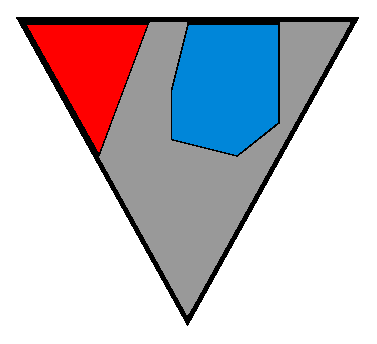
\includegraphics[width=\proofwidth]{figures/two_phase_draft_proof}
		}
		%\rule{0.4\textwidth}{0.1\textwidth}
		%\end{center}
		&
		\vspace*{0.2em}
		\\

		%& \begin{center} \large\stagearrow \end{center} & 
		%\multicolumn{2}{c}{\emph{Extract structure from proof}}
		\multicolumn{2}{l}{
			\proofindent{\stagearrow} ~\parbox[c]{14em}{\raggedright \emph{ Extract propositional interpolant structure from proof}}
			\vspace*{0.2em}
		}
		\\

		%&  \Huge\stagearrow}   \\

	\begin{tabular}[x]{@{}l@{}}Propositional\\Interpolant:\end{tabular} 
		%	Propositional \newline interpolant: 
		&
		%\begin{center} \end{center}
		%\rule{0.4\textwidth}{0.1\textwidth}
		\multicolumn{1}{m{\fakemulticolwidth}}{
			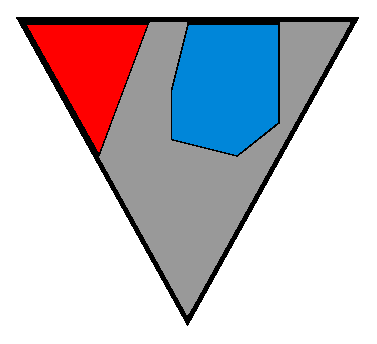
\includegraphics[width=\proofwidth]{figures/two_phase_draft_proof}
		}
		$\dots \gray Q(\colA f(\colB c), \colB c) \dots$
		\vspace*{0.2em}
		\\
		\multicolumn{2}{l}{
			\proofindent{\stagearrow} ~\parbox[c]{12em}{\raggedright \emph{ Replace colored function and constant symbols }}
			\vspace*{0.2em}
		}
		\\

	\begin{tabular}[x]{@{}l@{}}Prenex\\First-Order\\Interpolant:\end{tabular} 
		&
		\multicolumn{1}{m{\fakemulticolwidth}}{
			
\includegraphics[width=\proofwidth]{figures/two_phase_draft_fo_interpolant}
		}
		$\exists {x_3} \forall {x_5} \dots \gray Q({x_5}, {x_3}) \dots$
		\\


	\end{tabular}

\end{frame}

\subsection{}
\begin{frame}{Huang's algorithm (2/2)}
	\begin{itemize}
		\item Propositional interpolant is interpolant modulo function and constant symbols
		\item For the lifting phase, the ordering of the lifting variables is crucial
		\item The type of the quantifier is determined by the coloring of the symbol

			\pause

			\begin{theorem}
				The number of quantifier alternations in the resulting interpolant directly corresponds to the number of color alternations of terms in the resolution proof.
			\end{theorem}
	\end{itemize}
\end{frame}


\newcommand{\onePhaseArrowLabel}{Combined structure extraction and replacing of colored symbols}

\subsection{}
\begin{frame}{Interpolation extraction in one phase}
	\small
	\begin{tabular}{p{0.25\textwidth}ll}

		Proof: 
		&

		\multicolumn{1}{m{\fakemulticolwidth}}{
			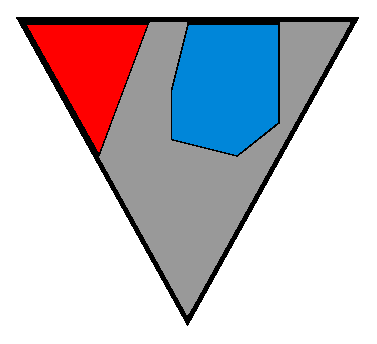
\includegraphics[width=\proofwidth]{figures/two_phase_draft_proof}
		}
		&
		\vspace*{0.2em}
		\\

		\multicolumn{2}{l}{
			\proofindent{\stagearrow} ~\parbox[c]{15em}{\raggedright\emph{ \onePhaseArrowLabel } }
			\vspace*{0.2em}
		}
		\\

	\begin{tabular}[x]{@{}l@{}}Interpolant\\modulo\\current clause:\end{tabular} 
		&
		\multicolumn{1}{m{\fakemulticolwidth}}{
			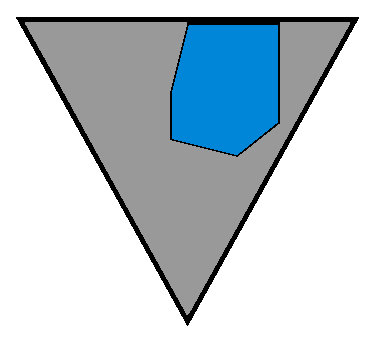
\includegraphics[width=\proofwidth]{figures/one_phase_draft_intermediate}
		}
		$\forall {x_5} \dots \gray Q({x_5}, \colB c) \dots$
		\vspace*{0.2em}
		\\

		\multicolumn{3}{l}{
			\hspace*{5em}
			\parbox[c]{13.3em}{\emph{Recursively applied to all inferences of the proof results in:}}
			%\proofindent{\stagearrow} ~\parbox[c]{15em}{\raggedright\emph{ \onePhaseArrowLabel } }
			%				\vspace*{0.5em}
			\vspace*{0.5em}
		}
		\\


		%			\multicolumn{2}{l}{
		%				\proofindent
		%				$\left.
		%				\parbox[c]{2em}{
		%					\stagearrow\\
		%					\hspace*{0.318em}$\vdots$ \\[0.27\baselineskip]
		%					\stagearrow
		%				}
		%			\right\} 
		%			\parbox[t]{11em}{\emph{Combined extraction and replacing phases}}
		%			$
		%				\vspace*{0.5em}
		%			} 
		%		 \\

	\begin{tabular}[x]{@{}l@{}}Non-Prenex\\First-Order\\Interpolant:\end{tabular} 
		&
		\multicolumn{1}{m{\fakemulticolwidth}}{
			
\includegraphics[width=\proofwidth]{figures/two_phase_draft_fo_interpolant}
		}
		$\exists {x_3} \dots \forall {x_5} \dots \gray Q({x_5}, {x_3}) \dots$
		\\



	\end{tabular}

\end{frame}

\section{Semantic Proof (6 min)}
\begin{frame}{Semantic Proof}

	TODO

\end{frame}

\section{Conclusion}
\begin{frame}{Conclusion}
	\begin{itemize}
		\item Craig's and Huang's proof based interpolant extraction from proofs

			$\Rightarrow$ differ in applicability 

		\item Craig shows that the interpolation theorem holds also in FOL/EQ
		\item Huang shows that interpolants can efficiently be extracted in FOL/EQ

			\begin{itemize}
				\item Does not require different methods
				\item Little attention so far in research
			\end{itemize}

		\item Interpolation also allows for a model theoretic approach

	\end{itemize}
\end{frame}

\subsection{References}
\begin{frame}
	\bibliography{bib}
\end{frame}

\end{document}
